\documentclass[ignorenonframetext,]{beamer}
\setbeamertemplate{caption}[numbered]
\setbeamertemplate{caption label separator}{: }
\setbeamercolor{caption name}{fg=normal text.fg}
\beamertemplatenavigationsymbolsempty
\usepackage{lmodern}
\usepackage{amssymb,amsmath}
\usepackage{ifxetex,ifluatex}
\usepackage{fixltx2e} % provides \textsubscript
\ifnum 0\ifxetex 1\fi\ifluatex 1\fi=0 % if pdftex
  \usepackage[T1]{fontenc}
  \usepackage[utf8]{inputenc}
\else % if luatex or xelatex
  \ifxetex
    \usepackage{mathspec}
  \else
    \usepackage{fontspec}
  \fi
  \defaultfontfeatures{Ligatures=TeX,Scale=MatchLowercase}
\fi
\usetheme[]{Berlin}
\usecolortheme{seagull}
\usefonttheme{structuresmallcapsserif}
% use upquote if available, for straight quotes in verbatim environments
\IfFileExists{upquote.sty}{\usepackage{upquote}}{}
% use microtype if available
\IfFileExists{microtype.sty}{%
\usepackage{microtype}
\UseMicrotypeSet[protrusion]{basicmath} % disable protrusion for tt fonts
}{}
\newif\ifbibliography
\hypersetup{
            pdftitle={Effectiveness of private sector malaria control: The case of sugarcane workers in Mozambique},
            pdfborder={0 0 0},
            breaklinks=true}
\urlstyle{same}  % don't use monospace font for urls
\usepackage{graphicx,grffile}
\makeatletter
\def\maxwidth{\ifdim\Gin@nat@width>\linewidth\linewidth\else\Gin@nat@width\fi}
\def\maxheight{\ifdim\Gin@nat@height>\textheight0.8\textheight\else\Gin@nat@height\fi}
\makeatother
% Scale images if necessary, so that they will not overflow the page
% margins by default, and it is still possible to overwrite the defaults
% using explicit options in \includegraphics[width, height, ...]{}
\setkeys{Gin}{width=\maxwidth,height=\maxheight,keepaspectratio}

% Prevent slide breaks in the middle of a paragraph:
\widowpenalties 1 10000
\raggedbottom

\AtBeginPart{
  \let\insertpartnumber\relax
  \let\partname\relax
  \frame{\partpage}
}
\AtBeginSection{
  \ifbibliography
  \else
    \let\insertsectionnumber\relax
    \let\sectionname\relax
    \frame{\sectionpage}
  \fi
}
\AtBeginSubsection{
  \let\insertsubsectionnumber\relax
  \let\subsectionname\relax
  \frame{\subsectionpage}
}

\setlength{\parindent}{0pt}
\setlength{\parskip}{6pt plus 2pt minus 1pt}
\setlength{\emergencystretch}{3em}  % prevent overfull lines
\providecommand{\tightlist}{%
  \setlength{\itemsep}{0pt}\setlength{\parskip}{0pt}}
\setcounter{secnumdepth}{0}
\usepackage{multicol}
\usepackage{hyperref}
\usepackage{geometry}
\usepackage[utf8]{inputenc}
% \usepackage[T1]{fontenc}
\usepackage{lmodern}
\pagenumbering{gobble}
\usepackage{longtable}
\usepackage{changepage}
\usepackage{graphicx}
\usepackage{multicol}
\usepackage{geometry}
\usepackage{color}
\usepackage{colortbl}
\usepackage{color}
% Font
\usepackage{fontspec}
\setmainfont{Swift-Regular_43151.ttf}
\setsansfont[BoldFont={Swift-Bold_43130.ttf}]{Swift-Regular_43151.ttf}
% \setmonofont{Swift-Regular_43151.ttf}
\renewcommand{\familydefault}{\sfdefault}
% \usepackage{fontspec}
% \setmainfont{Lato-Regular.ttf}
% \setsansfont[BoldFont={Lato-Bold.ttf}]{Lato-Regular.ttf}
% \renewcommand{\familydefault}{\sfdefault}

\def\changemargin#1#2{\list{}{\rightmargin#2\leftmargin#1}\item[]}
\let\endchangemargin=\endlist
\renewcommand{\rmdefault}{ppl}

\usepackage{multicol}
\usepackage{hyperref}
\usepackage{geometry}
\usepackage{lipsum}

% \usepackage{todonotes} % for side notes
% \usepackage[colorinlistoftodos]{todonotes} % for side notes

\usepackage{xargs}                      % Use more than one optional parameter in a new commands
% \usepackage[dvipsnames, table]% Coloured text etc.
% 
% \usepackage[colorinlistoftodos,prependcaption,textsize=tiny]{todonotes}
% \newcommandx{\unsure}[2][1=]{\todo[linecolor=red,backgroundcolor=red!25,bordercolor=red,#1]{#2}}
% \newcommandx{\change}[2][1=]{\todo[linecolor=blue,backgroundcolor=blue!25,bordercolor=blue,#1]{#2}}
% \newcommandx{\info}[2][1=]{\todo[linecolor=OliveGreen,backgroundcolor=OliveGreen!25,bordercolor=OliveGreen,#1]{#2}}
% \newcommandx{\improvement}[2][1=]{\todo[linecolor=Plum,backgroundcolor=Plum!25,bordercolor=Plum,#1]{#2}}
% \newcommandx{\thiswillnotshow}[2][1=]{\todo[disable,#1]{#2}}
% \usepackage{lmodern}

% \newcommand{\footremember}[2]{%
%     \footnote{#2}
%     \newcounter{#1}
%     \setcounter{#1}{\value{footnote}}%
% }
% \newcommand{\footrecall}[1]{%
%     \footnotemark[\value{#1}]%
% }

\def\changemargin#1#2{\list{}{\rightmargin#2\leftmargin#1}\item[]}
\let\endchangemargin=\endlist

\widowpenalties 1 150

\makeatletter
\renewcommand\footnotesize{%
   \@setfontsize\footnotesize\@ixpt{11}%
   \abovedisplayskip 8\p@ \@plus2\p@ \@minus4\p@
   \abovedisplayshortskip \z@ \@plus\p@
   \belowdisplayshortskip 4\p@ \@plus2\p@ \@minus2\p@
   \def\@listi{\leftmargin\leftmargini
               \topsep 4\p@ \@plus2\p@ \@minus2\p@
               \parsep 2\p@ \@plus\p@ \@minus\p@
               \itemsep \parsep}%
   \belowdisplayskip \abovedisplayskip
}
\makeatother

% \DeclareTextCommandDefault{\nobreakspace}{\leavevmode\nobreak\ } 



























\newcommand{\footremember}[2]{%
    \footnote{#2}
    \newcounter{#1}
    \setcounter{#1}{\value{footnote}}%
}
\newcommand{\footrecall}[1]{%
    \footnotemark[\value{#1}]%
}

% \def\changemargin#1#2{\list{}{\rightmargin#2\leftmargin#1}\item[]}
% \let\endchangemargin=\endlist

\widowpenalties 1 150


\makeatletter
\renewcommand\footnotesize{%
   \@setfontsize\footnotesize\@ixpt{7}%
   \abovedisplayskip 8\p@ \@plus2\p@ \@minus4\p@
   \abovedisplayshortskip \z@ \@plus\p@
   \belowdisplayshortskip 4\p@ \@plus2\p@ \@minus2\p@
   \def\@listi{\leftmargin\leftmargini
               \topsep 4\p@ \@plus2\p@ \@minus2\p@
               \parsep 2\p@ \@plus\p@ \@minus\p@
               \itemsep \parsep}%
   \belowdisplayskip \abovedisplayskip
}
\makeatother

\title{Effectiveness of private sector malaria control: The case of sugarcane
workers in Mozambique}
\subtitle{ISGlobal, Economics Group, Internal Meeting, March, 2018}
\date{}

\begin{document}
\frame{\titlepage}

\begin{frame}

Joe
Brew\footremember{isglobal}{Barcelona Institute for Global Health, Spain}\footremember{cism}{Centro de Investigação em Saúde de Manhiça, Mozambique}\footremember{vu}{VU University Amsterdam, Netherlands}
\footnote{Corresponding Author}

Kizito
Gondo\footremember{ma}{Maragra Açucar SA, Subsidiary of Illovo Sugar Ltd, Mozambique}

Elton Dorkin\footrecall{ma}

Eduardo Nhamahanga\footrecall{ma}

Menno
Pradhan\footrecall{vu}\footremember{uva}{University of Amsterdam, Netherlands}

Laia Cirera\footrecall{isglobal}\footrecall{cism}

Ranjeeta Thomas\footremember{icl}{Imperial College London, UK}

Elisa Sicuri\footrecall{isglobal}\footrecall{cism}\footrecall{icl}

\end{frame}

\section{Introduction}\label{introduction}

\begin{frame}{Abstract}

This paper provides new empirical evidence regarding the return on
investment of privately managed malaria control activities (indoor
residual spraying with pesticides) on worker absenteeism in Mozambique.
We analyze 4 years of malaria control and worker health and absenteeism
data from a large sugar processing facility in Mozambique. We find that
the benefits outweight the costs (ie, there is a positive return on
investment) even when the consideration of benefits is limited to those
directly accrued by the company. These findings suggest that the private
sector may have an important role to play in malaria control in endemic
areas.

\end{frame}

\begin{frame}{Overview}

\begin{block}{Research highlights}

\begin{itemize}
\tightlist
\item
  Large, individual-level worker absenteeism data from malaria endemic
  zone\\
\item
  Quantifies effect of indoor residual spraying on absenteeism\\
\item
  Estimates cost-effectiveness of malaria control from investment
  standpoint\\
\item
  Results suggest that private sector could play a significant role in
  malaria elimination
\end{itemize}

\end{block}

\begin{block}{Keywords}

Malaria; Investment; Health; Productivity; Agriculture; Absenteeism

\end{block}

\end{frame}

\begin{frame}{Context}

\begin{itemize}
\tightlist
\item
  Malaria has a large economic impact on endemic societies. By affecting
  saving, investment (Shretta, Avanceña, and Hatefi 2016), risk
  perception, productivity, absenteeism (Nonvignon et al. 2016), human
  capital accumulation (Castel-Branco 2014), mortality, and costs of
  care (Sachs and Malaney 2002), malaria likely has a negative effect on
  GDP and growth (McCarthy, Wolf, and Wu 2000) (Orem et al. 2012).\\
\item
  Because of the relative affordability of most intereventions and the
  enormous societal costs of malaria, most forms of malaria control are
  cost-effective when a public welfare perspective is assumed, such as
  when a government provides the financing (White et al. 2011) (Purdy et
  al. 2013) (Howard et al. 2017).
\end{itemize}

\end{frame}

\begin{frame}{What we already know}

\begin{itemize}
\tightlist
\item
  Malaria is associated with absenteeism in workers (Nonvignon et al.
  2016).
\item
  Malaria has a negative effect on GDP (Orem et al. 2012) and growth
  (McCarthy, Wolf, and Wu 2000).
\item
  Malaria control is cost-effective from the societal/public perspective
  (Purdy et al. 2013).
\item
  Indoor residual spraying (IRS) is cost-effective (Howard et al. 2017),
  (White et al. 2011) \emph{from a public perspective}.
\end{itemize}

\end{frame}

\begin{frame}{What we want to know}

What is the investment case \emph{from the investor's perspective}?

\begin{itemize}
\tightlist
\item
  Is malaria control just good ``corporate social responsibility''? Or
  is it also good business?
\item
  From a purely financial/investment point-of-view, what benefits does a
  private company experience in engaging in malaria control?\\
\item
  What is the short-term \textbf{benefits} of IRS for large companies in
  malaria-endemic regions?
\item
  What are the \textbf{costs} of of carrying out IRS for large
  companies?
\end{itemize}

\end{frame}

\begin{frame}{What is already known from the private sector
perspective?}

\begin{itemize}
\tightlist
\item
  Public health interventions targetting malaria - and their
  corresponding cost-effectiveness evaluations - most often focus on
  impacts pertaining to public welfare, such as an increase in life
  years adjusted for disability or quality (Goodman, Coleman, and Mills
  1999) (Shretta, Avanceña, and Hatefi 2016) (Lee et al. 2017) (Hanson
  2004).\\
\item
  Though population-level health is certainly of importance to
  businesses, and improvements in health incidentally improve the
  economy at all levels (Brundtland 1999) (Bloom and Canning 2008)
  (Vecchi, Hellowell, and Gatti 2013), these improvements may be too
  disperse or long-term to incentivize private sector involvement in
  health campaigns.
\end{itemize}

\end{frame}

\begin{frame}{Mozambique}

\begin{itemize}
\tightlist
\item
  100\% of the Mozambican population are at risk of malaria, living in
  what the WHO classifies as a ``high transmission'' area (Moonasar et
  al. 2016).\\
\item
  Annually, Mozambique has more than 8 million clinical malaria cases
  (an annual incidence of approximately 300 per 1,000 residents), with
  an estimated 14,000 deaths.\\
\item
  Malaria accounts for 29\% of all deaths, and 42\% of deaths among
  those under five years of age (INE 2011).\\
\item
  Since 2013, Mozambique has seen a gradual increase in the incidence of
  malaria (Moonasar et al. 2016).\\
\item
  100\% of the malaria in Mozambique is of the Plasmodium falciparum
  species, with Anopheles funestus, gambiae, and arabiensis as the
  primary mosquito vectors of the disease (WHO 2015).
\end{itemize}

\end{frame}

\begin{frame}{Industry in Mozambique}

A significant sector of the economy in Mozambique is dominated by a full
large-scale foreing direct investment projects (Robbins and Perkins
2012), and the role of the private sector in health generally, and
malaria specifically, is unequivocally important.\\
- Large agriculture and extractive industry firms take up wide swaths of
land and employ hundreds of thousands (German, Schoneveld, and Mwangi
2013).\\
- The Mozambican state has encouraged large-scale entreprise with the
aim of general economic development (Buur, Tembe, and Baloi 2012).\\
- And where large firms exist, they often take on social roles such as
housing and health care (Winkler 2013) (Robbins and Perkins 2012)
(Castel-Branco 2014).

\end{frame}

\begin{frame}{Research questions}

\textbf{What is the short-term effect of IRS on worker absenteeism and
clinical illness among sugarcane workers?}

\end{frame}

\begin{frame}{Research site}

\includegraphics{internal_march_2018_files/figure-beamer/unnamed-chunk-4-1.pdf}

\end{frame}

\begin{frame}{Research Site II}

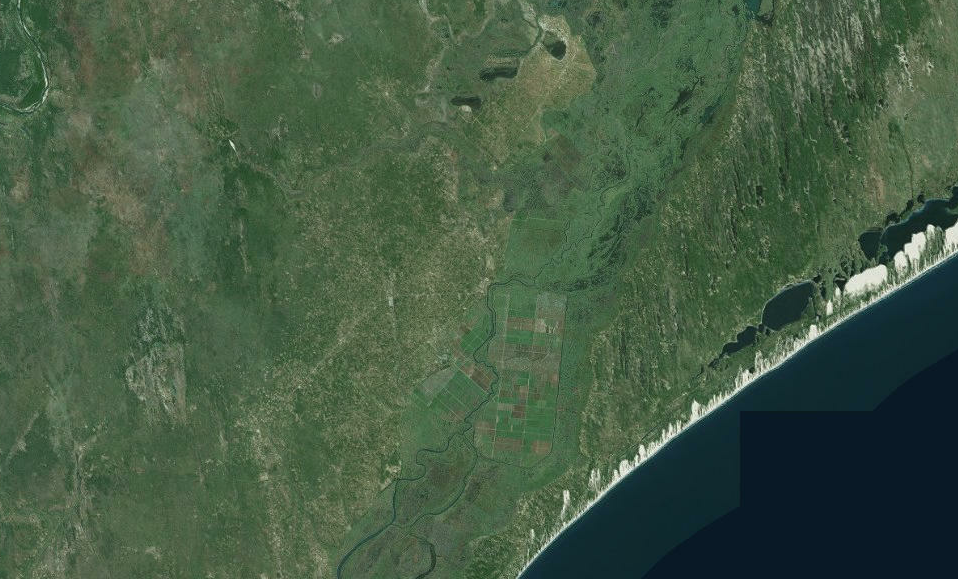
\includegraphics{images/sat}

\end{frame}

\section{Methods}\label{methods}

\begin{frame}{Data collection}

\begin{itemize}
\tightlist
\item
  January 2010 through December 2016.\\
\item
  Data came from four sources: (i) the Human Resources' roster of worker
  details and absences, (ii) the facility's on-site clinic's medical and
  laboratory records, (iii) the facility's on-site malaria control
  program's records pertaining to the dates, chemicals, and location of
  IRS activities, and (iv) interviews with company employees pertaining
  to costs, data limitations, etc.\\
\item
  Digitization and collection of data took place during the period from
  March 2016 through May 2017.
\item
  Supplementary data from through the Centro de Investigação em Saude de
  Manhiça's (CISM) (Nhacolo et al. 2006).
\end{itemize}

\end{frame}

\begin{frame}{Epidemiological data}

\begin{itemize}
\tightlist
\item
  District-wide malaria incidence was obtained from Mozambique's Boletim
  Epidemiológico Semanal (BES)\\
\item
  Weather data for all Mozambican stations from NOAA.
\end{itemize}

\end{frame}

\begin{frame}{Comment on intervention target groups}

Maragra regularly employs IRS at on-site worker households in order to
reduce those workers' (and their families') risk of malaria infection.
Workers living off-site (our control group) also may have received IRS
at some point during the study period (from government programs). Even
though we do not have reliable person-level data on IRS carried out by
the government, off-site workers are a suitable control in the sense
that they represent ``business as usual'' (ie, what would happen if the
company carried out no IRS and relied solely on public interventions).
Using company HR and clinical records, we were able to identify absences
and episodes of clinical malaria among all workers, as well as identify
the time since the most recent IRS episode before the onsent of absence
or illness.

\end{frame}

\begin{frame}{Conceptual framework and identification strategy}

We sought to understand the effect of IRS on individual workers'
likelihood of absence from work as well as their likelihood of clinical
malaria. To estimate this effect, we estimated separate models for
absence and illness. We employed interrupted time series (Lopez Bernal,
Cummins, and Gasparrini 2016) and a linear probability approach using
the following econometric model.

\[
\hat{Y_{it}} = \beta_{0} +  (\beta_{1}) (\text{Season}_{t}) + (\beta_2{IRS}*\beta_3{IRS_t}) + ... + \epsilon
\]

\(\hat{Y}\) is the rate of absence. \(\beta_{1}\) represents the
clinical malaria incidence at that time in the entire district of
Manhiça. Our demographic confounders (represented by \(...\)) are sex,
age, and worker department (field, factory, or administrative).

\end{frame}

\begin{frame}{More model details}

\begin{itemize}
\tightlist
\item
  Intervention not a simple yes/no: (\(_t\)) represents time elapsed
  since commencement of the most recent IRS campaign).\\
\item
  ``Malaria season'': clinical incidence of malaria in the district of
  Manhiça was at or greater than the median clinical incidence of
  malaria for the entire study period.\\
\item
  By using clinical incidence of the area of residence of the workers
  (as opposed to more typical proxies for malaria risk, such as only
  rainy vs.~non rainy season), our seasonality estimate is a closer
  approximation of true malaria risk, incorporating lagged effects such
  as the incubation period of the parasite, as well as any inherent
  non-linear effects of weather.
\end{itemize}

\end{frame}

\begin{frame}{Estimating return on investment}

Our formula for return on investment can be described in a
straightforward fashion\ldots{}

\begin{center}
$R = \dfrac{P_{w} - S_{wa} - S_{wc}}{P_{w}}$

\end{center}

\ldots{}where \(R\) is the return on investment, \(P\) is the malaria
control program's total operating cost, \(w\) refers to costs at the
per-worker level, \(a\) refers to savings through avoided absences, and
\$ c \$ refers to savings through avoided clinical encounters. We define
the malaria control program as ``profitable'' from an investment
standpoint if ROI is greater than 100\%, ie if the savings associated
with the estimated effect of IRS is greater than the costs of the
program's administration.

\end{frame}

\begin{frame}{Reproducibility and ethical approval}

All data processing and analysis were carried out in R (R Core Team
2017) and all analysis code is freely available online (Brew 2017).
Ethical approval for this project was obtained from the Institutional
Ethics Review Board for Health at the CISM prior to data collection.

\end{frame}

\section{Results}\label{results}

\begin{frame}{Descriptive overview}

\begin{figure}
\centering
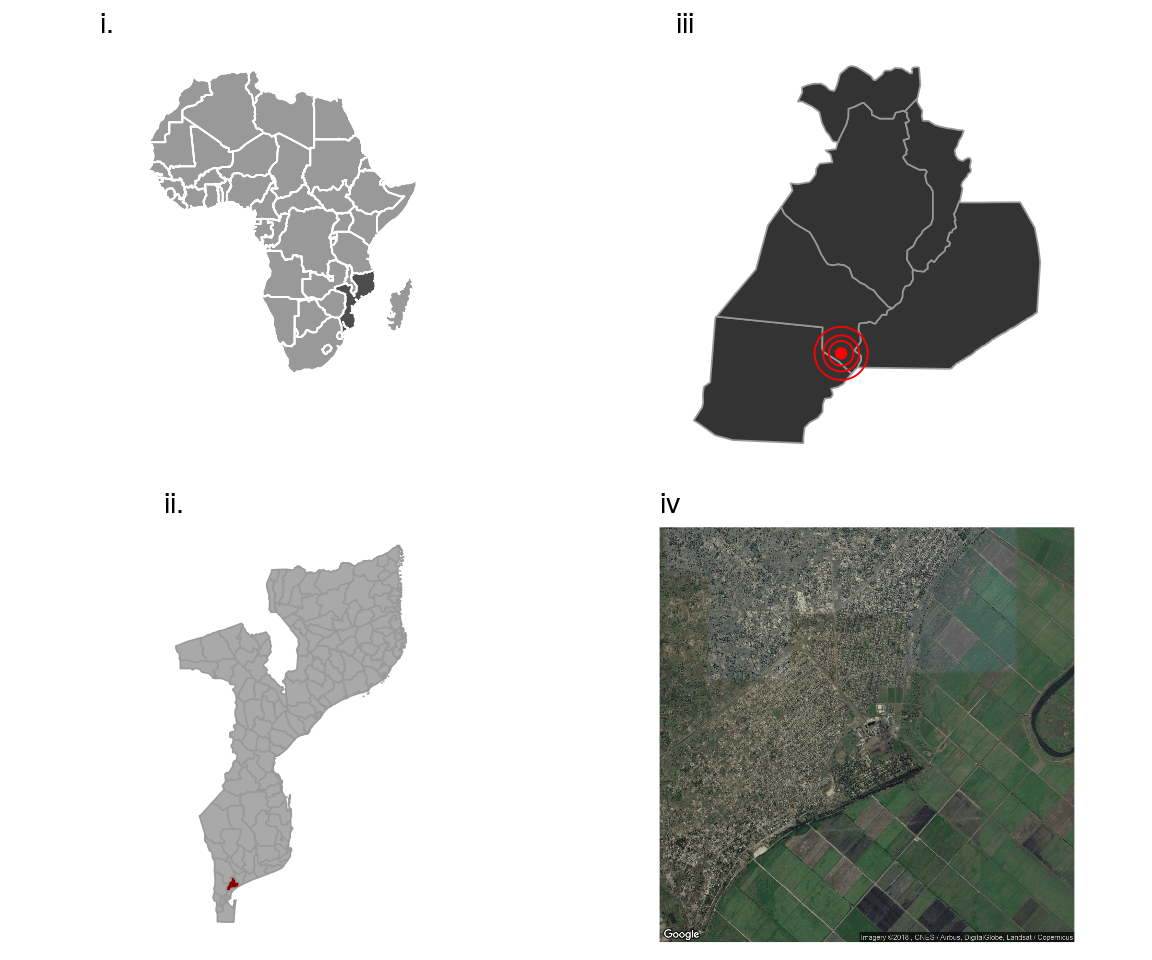
\includegraphics{internal_march_2018_files/figure-beamer/unnamed-chunk-5-1.pdf}
\caption{Clinical malaria (district of Manhiça), all-cause absenteeism
among Maragra workers, sick absenteeism among Maragra workers, estimated
rainfall, positive cases at company clinic, and test positivity rate at
company clinic}
\end{figure}

\end{frame}

\begin{frame}{Descriptive: absenteeism by time from/to intervention}

\includegraphics{internal_march_2018_files/figure-beamer/unnamed-chunk-6-1.pdf}

\end{frame}

\begin{frame}{Descriptive: absenteeism by time from/to intervention
(with local regression lines)}

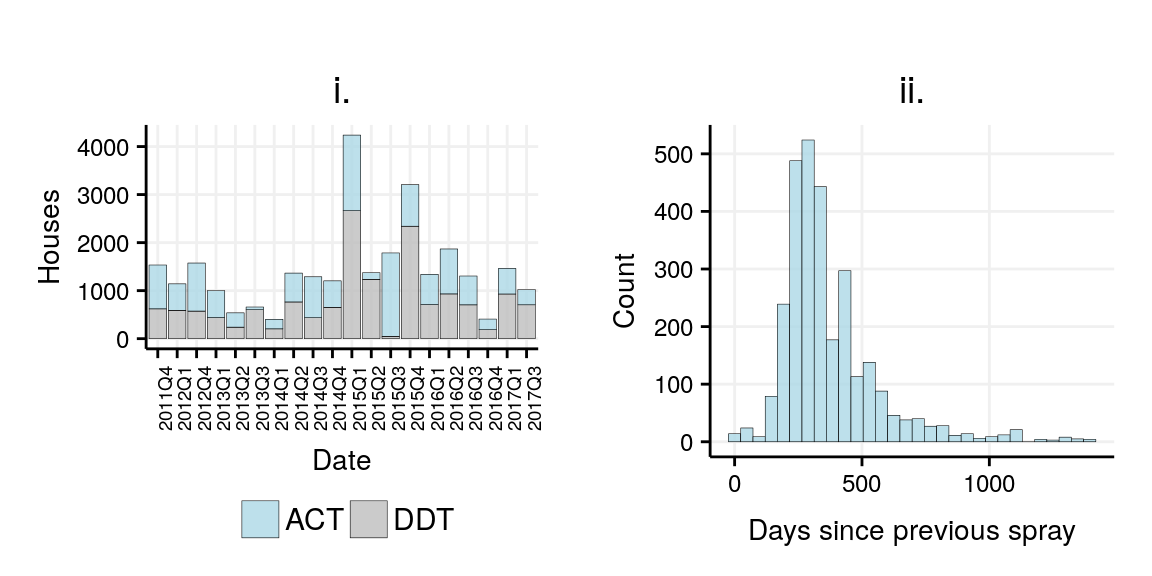
\includegraphics{internal_march_2018_files/figure-beamer/unnamed-chunk-7-1.pdf}

\end{frame}

\begin{frame}{Descriptive: absenteeism by time from/to intervention (by
time period)}

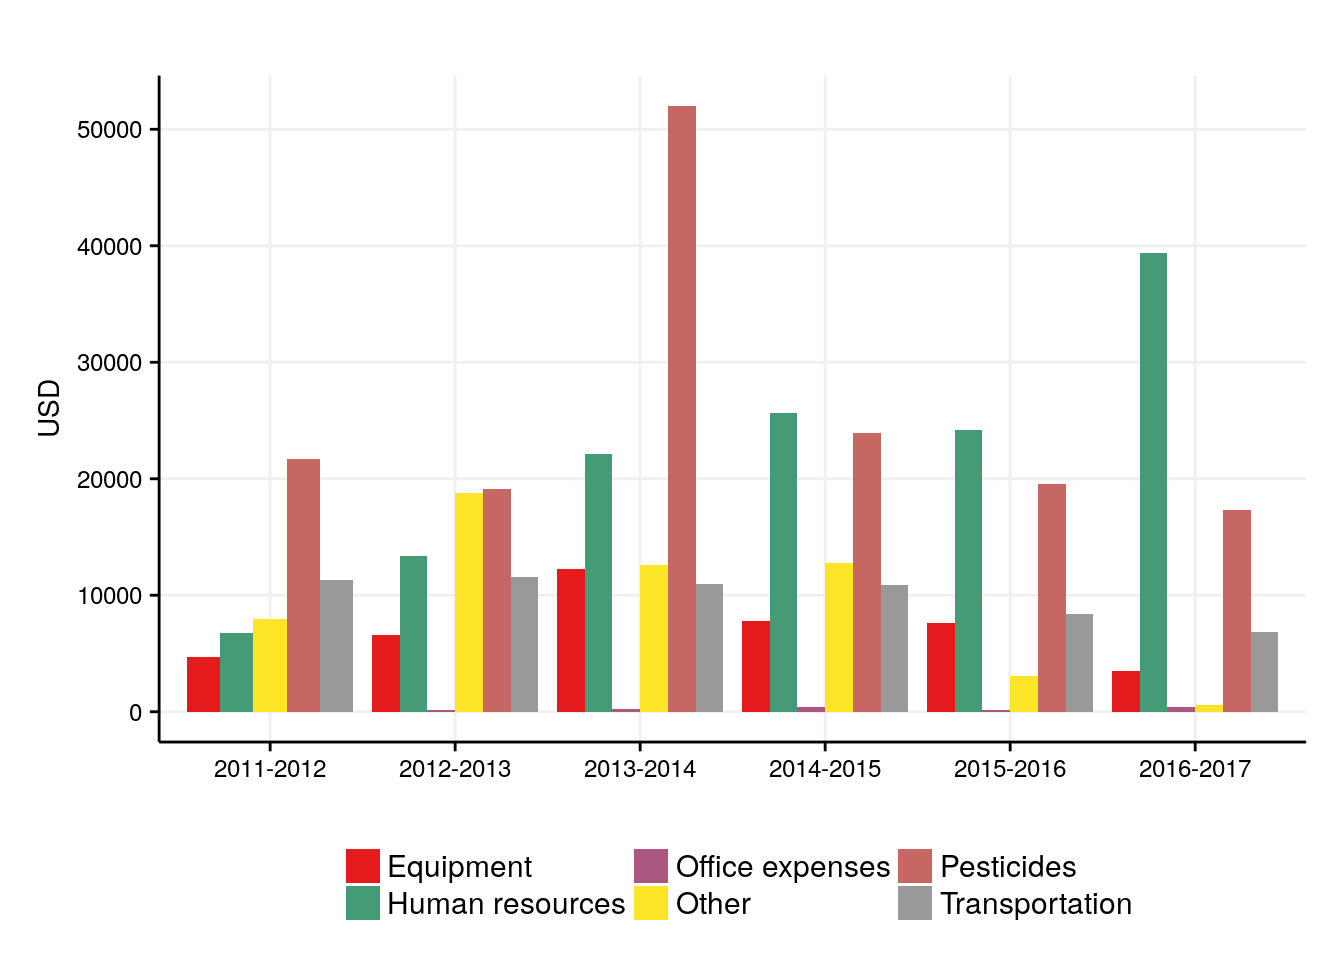
\includegraphics{internal_march_2018_files/figure-beamer/unnamed-chunk-8-1.pdf}

\end{frame}

\begin{frame}{Same chart with local regression lines}

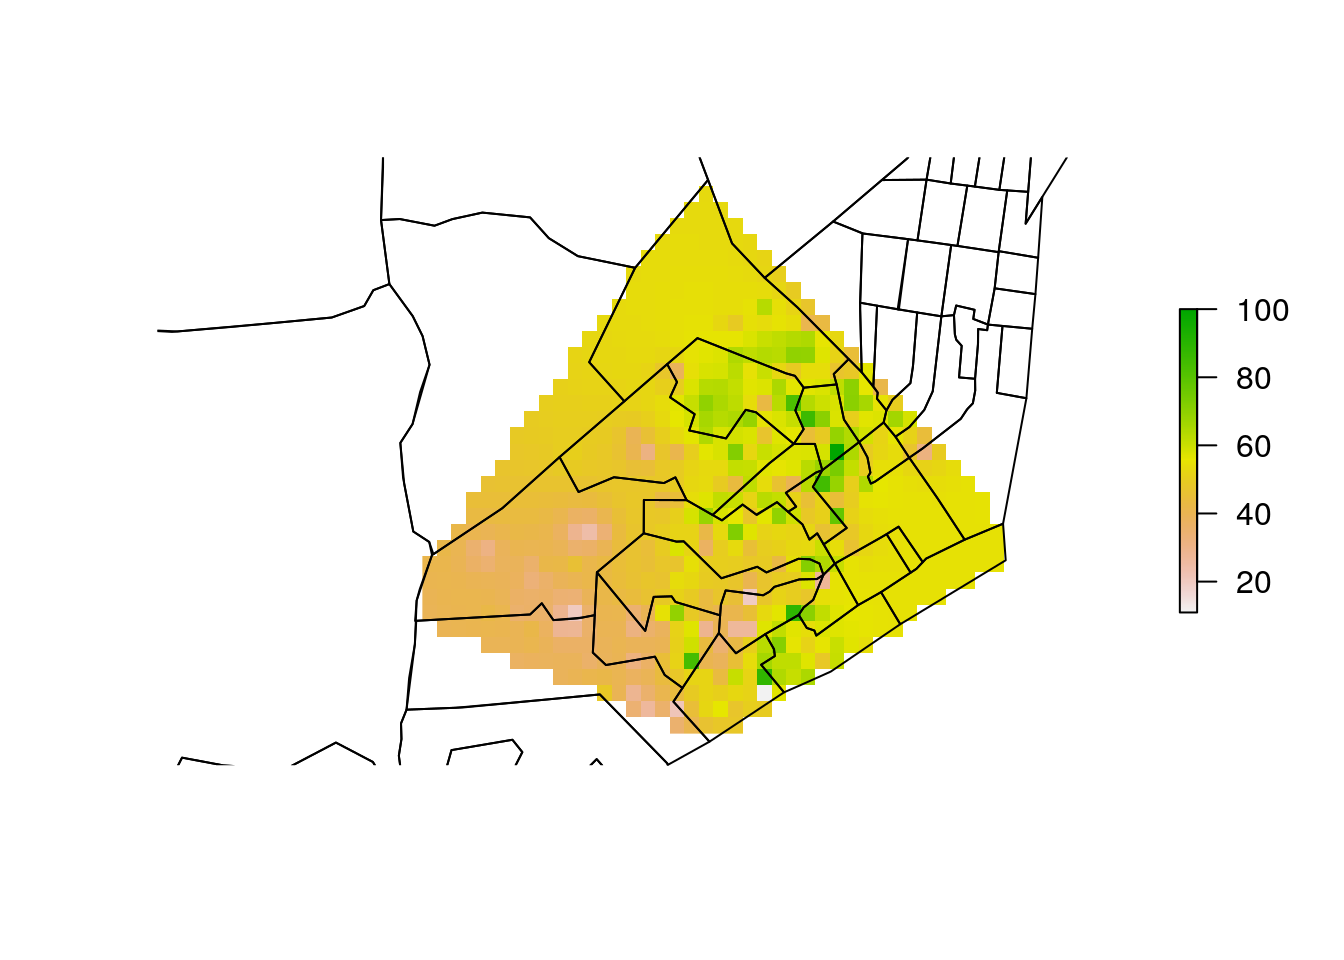
\includegraphics{internal_march_2018_files/figure-beamer/unnamed-chunk-9-1.pdf}

\end{frame}

\begin{frame}{Descriptive: absenteeism in binned time period}

\includegraphics{internal_march_2018_files/figure-beamer/unnamed-chunk-10-1.pdf}

\end{frame}

\begin{frame}{Descriptive: absenteeism in binned time periods by season}

\includegraphics{internal_march_2018_files/figure-beamer/unnamed-chunk-11-1.pdf}

\end{frame}

\begin{frame}{Costs}

The malaria control program at Maragra has an annual operating budget of
approximately XX, which includes the purchase of insecticide, the wages
of IRS sprayers and drivers, transportation, record-keeping, and general
administrative costs. Assuming linearity in costs, the program spends
approximately XX per agregado sprayed. With each agregado containing an
average of 2.2 workers, this translates to a cost of XX per worker
protected per season. Much of the benefit of IRS goes to non-worker
residents of sprayed agregados (who constitute a majority), but this
benefit is purposefully ignored for this analysis.

\end{frame}

\begin{frame}{Savings}

Given the likelihood that clinical data does not fully capture all
malaria cases, we do not quantify the costs of malaria infection to the
company. Rather, we first estimate the reduction in absenteeism
attributible to IRS, and then quantify the savings associated with
prevented absences. Additionally, we calculate the clinical savings of
IRS by first estimating the share of absences which are associated with
an episode of clinical malaria, and then applying the clinical cost per
case to the equivalent share of prevented absences. We intentionally
ignore the savings accrued by the public health system, as well as the
likely utility gains in secondary realms such as school absenteeism,
producitivity, etc.

\end{frame}

\begin{frame}{Effect of IRS on absenteeism}

\begin{itemize}
\tightlist
\item
  IRS is associated with a year-long, significant reduction in
  absenteeism during the malaria season.\\
\item
  As one would expect if the mechanism by which IRS reduces absence is
  through reduced malaria infection, the effect of IRS during the low
  transmission season is significant, but far less substantial in effect
  size.
\end{itemize}

\end{frame}

\begin{frame}{Fixed effects models}

We create 4 worker fixed effects models. Different models for field vs
not field, permanent vs temporary.

\end{frame}

\begin{frame}{Fixed effects models (1)}

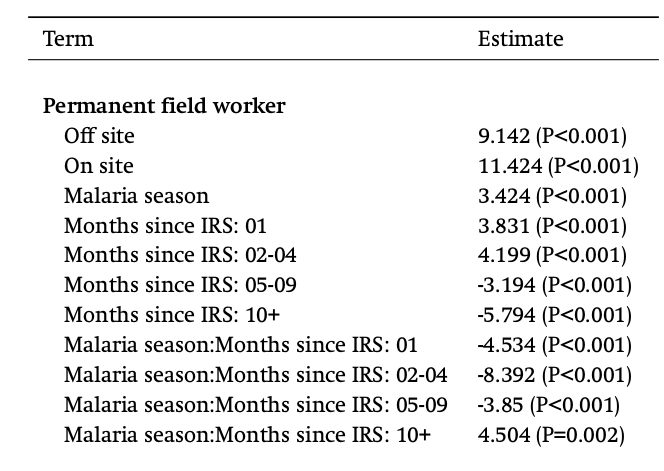
\includegraphics{images/fe1.png}

\end{frame}

\begin{frame}{Fixed effects models (2)}

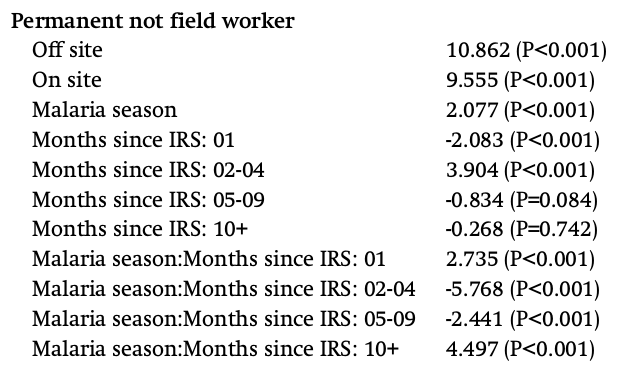
\includegraphics{images/fe2.png}

\end{frame}

\begin{frame}{Fixed effects models (3)}

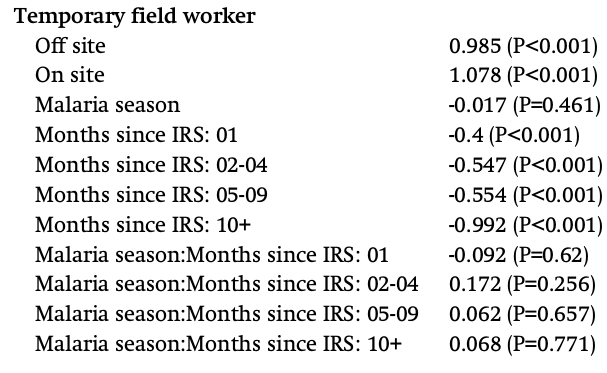
\includegraphics{images/fe3.png}

\end{frame}

\begin{frame}{Fixed effects models (4)}

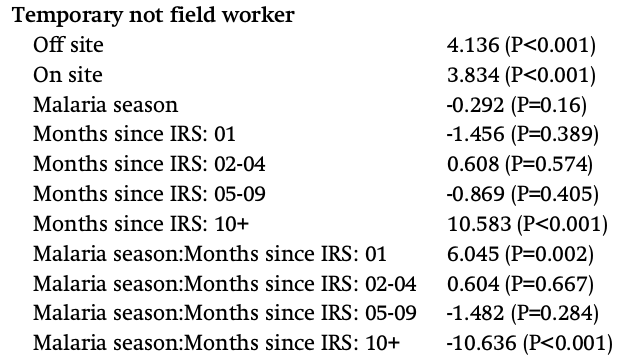
\includegraphics{images/fe4.png}

\end{frame}

\begin{frame}{Return on investment}

Details here on ROI calculation outcomes to go here.

\end{frame}

\begin{frame}{Back of envelope}

\textbf{Savings}

\begin{itemize}
\tightlist
\item
  In percentage point terms, reduction from 13\% to 8\%.\\
\item
  5 annually prevented absences per worker.\\
\item
  8,000 workers: 40,000 prevented absences, wage of 3 USD
\item
  TOTAL: 120,000 USD in productivity-only savings.
\end{itemize}

\textbf{Costs}

\begin{itemize}
\tightlist
\item
  8 IRS workers, 1500 USD yearly = 12,000 USD\\
\item
  ACT + DDT: 50,000 USD
\item
  Facilities, vehicles, gas: 50,000 USD\\
\item
  TOTAL: 112,000 USD in IRS-only costs
\end{itemize}

\textbf{7\% ROI} (ignoring clinical costs)

\end{frame}

\section{Discussion}\label{discussion}

\begin{frame}{General}

\begin{itemize}
\tightlist
\item
  30-50\% reduction in absenteeism in the 6 months after IRS during
  malaria season.
\item
  Depending on detailed cost data (pending), IRS may be effective even
  from a purely financial point of view (ie, beyond just ``corporate
  social responsibility'').\\
\item
  Next steps are incorporation of (a) productivity data (via cane cut),
  (b) better clinical data (via local health facilities), and (c) full
  cost data.\\
\item
  Will also be comparing with a sugarcane facility in a zone where an
  elimination campaign is taking place.
\end{itemize}

\end{frame}

\begin{frame}{Limitations}

\begin{itemize}
\tightlist
\item
  No analysis yet of different worker types (agricultural
  vs.~industrial).
\item
  Have not yet ventured at all into side-analyses (effect on employment,
  tonnage, etc.).
\item
  Sick absenteeism seems to track absenteeism poorly: lack of clarity
  regarding pathways.\\
\item
  Large sample size, but all from same place: questionable
  generalizability.
\end{itemize}

\end{frame}

\begin{frame}{Thank you}

\textbf{Email:}
\href{mailto:joe@economicsofmalaria.com}{\nolinkurl{joe@economicsofmalaria.com}}

\textbf{Paper:}
\href{http://economicsofmalaria.com/maragra.pdf}{economicsofmalaria.com/maragra.pdf}

\textbf{Presentation:}
\href{http://economicsofmalaria.com/maragraslides.pdf}{economicsofmalaria.com/maragraslides.pdf}

\end{frame}

\begin{frame}[allowframebreaks]{References}

\hypertarget{refs}{}
\hypertarget{ref-Bloom2008}{}
Bloom, David, and David Canning. 2008. ``Population Health and Economic
Growth,'' 1--25.

\hypertarget{ref-brewgit}{}
Brew, J.R. 2017. ``Malaria and Sugar: An in-Depth Examination of the
Effect of Malaria Control Activities on the Health and Productivity of
Maragra Sugarcane Factory Workers.'' \emph{GitHub Repository}.
\url{https://github.com/joebrew/maragra}; GitHub.

\hypertarget{ref-World1999}{}
Brundtland, Gro Harlem. 1999. ``WHO on Health and Economic
Productivity'' 25 (2): 396--402.

\hypertarget{ref-Buur2012}{}
Buur, Lars, Carlota Mondlane Tembe, and Obede Baloi. 2012. ``The White
Gold: The Role of Government and State in Rehabilitating the Sugar
Industry in Mozambique.'' \emph{Journal of Development Studies} 48 (3).
Informa UK Limited: 349--62.
doi:\href{https://doi.org/10.1080/00220388.2011.635200}{10.1080/00220388.2011.635200}.

\hypertarget{ref-CastelBranco2014}{}
Castel-Branco, Carlos Nuno. 2014. ``Growth, Capital Accumulation and
Economic Porosity in Mozambique: Social Losses, Private Gains.''
\emph{Review of African Political Economy} 41 (sup1). Informa UK
Limited: S26--S48.
doi:\href{https://doi.org/10.1080/03056244.2014.976363}{10.1080/03056244.2014.976363}.

\hypertarget{ref-German2013}{}
German, Laura, George Schoneveld, and Esther Mwangi. 2013.
``Contemporary Processes of Large-Scale Land Acquisition in Sub-Saharan
Africa: Legal Deficiency or Elite Capture of the Rule of Law?''
\emph{World Development} 48 (August). Elsevier BV: 1--18.
doi:\href{https://doi.org/10.1016/j.worlddev.2013.03.006}{10.1016/j.worlddev.2013.03.006}.

\hypertarget{ref-Goodman1999}{}
Goodman, CA, PG Coleman, and AJ Mills. 1999. ``Cost-Effectiveness of
Malaria Control in Sub-Saharan Africa.'' \emph{The Lancet} 354 (9176).
Elsevier BV: 378--85.
doi:\href{https://doi.org/10.1016/s0140-6736(99)02141-8}{10.1016/s0140-6736(99)02141-8}.

\hypertarget{ref-Hanson2004}{}
Hanson, K. 2004. ``Public and Private Roles in Malaria Control: The
Contributions of Economic Analysis.'' \emph{The American Journal of
Tropical Medicine and Hygiene} 71 (9176). The American Society of
Tropical Medicine; Hygiene: 168--73.
\url{http://www.ajtmh.org/docserver/fulltext/14761645/71/2_suppl/0700168.pdf?expires=1503070750\&id=id\&accname=guest\&checksum=F969ACD7BE7E3A5D929D87EEA8A6EA2B}.

\hypertarget{ref-Howard_2017}{}
Howard, Natasha, Lorna Guinness, Mark Rowland, Naeem Durrani, and
Kristian S. Hansen. 2017. ``Cost-Effectiveness of Adding Indoor Residual
Spraying to Case Management in Afghan Refugee Settlements in Northwest
Pakistan During a Prolonged Malaria Epidemic.'' Edited by Guilherme
S.Editor Ribeiro. \emph{PLOS Neglected Tropical Diseases} 11 (10).
Public Library of Science (PLoS): e0005935.
doi:\href{https://doi.org/10.1371/journal.pntd.0005935}{10.1371/journal.pntd.0005935}.

\hypertarget{ref-estatistica2009}{}
INE. 2011. ``Demographic Health Survey.'' \url{http://www.ine.gov.mz/}.

\hypertarget{ref-Lee2017}{}
Lee, Bruce Y., Eli Zenkov, Chandrani Chatterjee, Baltazar Candrinho,
Shufang Zhang, James Colborn, Olivier J. T. Briët, et al. 2017. ``The
Economic Value of Long-Lasting Insecticidal Nets and Indoor Residual
Spraying Implementation in Mozambique.'' \emph{The American Journal of
Tropical Medicine and Hygiene} 96 (6). American Society of Tropical
Medicine; Hygiene: 1430--40.
doi:\href{https://doi.org/10.4269/ajtmh.16-0744}{10.4269/ajtmh.16-0744}.

\hypertarget{ref-Lopez_Bernal_2016}{}
Lopez Bernal, James, Steven Cummins, and Antonio Gasparrini. 2016.
``Interrupted Time Series Regression for the Evaluation of Public Health
Interventions: A Tutorial.'' \emph{International Journal of
Epidemiology}, June. Oxford University Press (OUP), dyw098.
doi:\href{https://doi.org/10.1093/ije/dyw098}{10.1093/ije/dyw098}.

\hypertarget{ref-McCarthy_2000}{}
McCarthy, Desmond, Holger Wolf, and Yi Wu. 2000. ``The Growth Costs of
Malaria,'' February. National Bureau of Economic Research.
doi:\href{https://doi.org/10.3386/w7541}{10.3386/w7541}.

\hypertarget{ref-Moonasar_2016}{}
Moonasar, Devanand, Rajendra Maharaj, Simon Kunene, Baltazar Candrinho,
Francisco Saute, Nyasatu Ntshalintshali, and Natashia Morris. 2016.
``Towards Malaria Elimination in the Mosaswa (Mozambique, South Africa
and Swaziland) Region.'' \emph{Malaria Journal} 15 (1). Springer Nature.
doi:\href{https://doi.org/10.1186/s12936-016-1470-8}{10.1186/s12936-016-1470-8}.

\hypertarget{ref-Nhacolo_2006}{}
Nhacolo, Ariel Q, Delino A Nhalungo, Charfudin N Sacoor, John J Aponte,
Ricardo Thompson, and Pedro Alonso. 2006. ``Levels and Trends of
Demographic Indices in Southern Rural Mozambique: Evidence from
Demographic Surveillance in Manhiça District.'' \emph{BMC Public Health}
6 (1). Springer Nature.
doi:\href{https://doi.org/10.1186/1471-2458-6-291}{10.1186/1471-2458-6-291}.

\hypertarget{ref-Nonvignon_2016}{}
Nonvignon, Justice, Genevieve Cecilia Aryeetey, Keziah L. Malm, Samuel
Agyei Agyemang, Vivian N. A. Aubyn, Nana Yaw Peprah, Constance N.
Bart-Plange, and Moses Aikins. 2016. ``Economic Burden of Malaria on
Businesses in Ghana: A Case for Private Sector Investment in Malaria
Control.'' \emph{Malaria Journal} 15 (1). Springer Nature.
doi:\href{https://doi.org/10.1186/s12936-016-1506-0}{10.1186/s12936-016-1506-0}.

\hypertarget{ref-Orem_2012}{}
Orem, Juliet, Joses Kirigia, Robert Azairwe, Ibrahim Kasirye, and
Oladapo Walker. 2012. ``Impact of Malaria Morbidity on Gross Domestic
Product in Uganda.'' \emph{International Archives of Medicine} 5 (1).
Springer Nature: 12.
doi:\href{https://doi.org/10.1186/1755-7682-5-12}{10.1186/1755-7682-5-12}.

\hypertarget{ref-Purdy_2013}{}
Purdy, Mark, David Rublin, Kuangyi Wei, and Matthew Robinson. 2013.
``The Economic Case for Combating Malaria.'' \emph{The American Journal
of Tropical Medicine and Hygiene} 89 (5). American Society of Tropical
Medicine; Hygiene: 819--23.
doi:\href{https://doi.org/10.4269/ajtmh.12-0689}{10.4269/ajtmh.12-0689}.

\hypertarget{ref-R}{}
R Core Team. 2017. \emph{R: A Language and Environment for Statistical
Computing}. Vienna, Austria: R Foundation for Statistical Computing.
\url{https://www.R-project.org/}.

\hypertarget{ref-Robbins2012}{}
Robbins, Glen, and David Perkins. 2012. ``Mining Fdi and Infrastructure
Development on Africa's East Coast: Examining the Recent Experience of
Tanzania and Mozambique.'' \emph{Journal of International Development}
24 (2). Wiley-Blackwell: 220--36.
doi:\href{https://doi.org/10.1002/jid.2817}{10.1002/jid.2817}.

\hypertarget{ref-Sachs2002}{}
Sachs, Jeffrey, and Pia Malaney. 2002. ``The Economic and Social Burden
of Malaria.'' \emph{Nature} 415 (6872). Springer Nature: 680--85.
doi:\href{https://doi.org/10.1038/415680a}{10.1038/415680a}.

\hypertarget{ref-Shretta2016}{}
Shretta, Rima, Anton L. V. Avanceña, and Arian Hatefi. 2016. ``The
Economics of Malaria Control and Elimination: A Systematic Review.''
\emph{Malaria Journal} 15 (1). Springer Nature.
doi:\href{https://doi.org/10.1186/s12936-016-1635-5}{10.1186/s12936-016-1635-5}.

\hypertarget{ref-Vecchi_2013}{}
Vecchi, Veronica, Mark Hellowell, and Stefano Gatti. 2013. ``Does the
Private Sector Receive an Excessive Return from Investments in Health
Care Infrastructure Projects? Evidence from the Uk.'' \emph{Health
Policy} 110 (2-3). Elsevier BV: 243--70.
doi:\href{https://doi.org/10.1016/j.healthpol.2012.12.010}{10.1016/j.healthpol.2012.12.010}.

\hypertarget{ref-White_2011}{}
White, Michael T, Lesong Conteh, Richard Cibulskis, and Azra C Ghani.
2011. ``Costs and Cost-Effectiveness of Malaria Control Interventions -
a Systematic Review.'' \emph{Malaria Journal} 10 (1). Springer Nature:
337.
doi:\href{https://doi.org/10.1186/1475-2875-10-337}{10.1186/1475-2875-10-337}.

\hypertarget{ref-whoprof}{}
WHO. 2015. ``Malaria Profile: Mozambique.'' World Health Organization.
\url{http://www.who.int/malaria/publications/country-profiles/profile_moz_en.pdf}.

\hypertarget{ref-Winkler}{}
Winkler, Deborah. 2013. ``Potential and Actual FDI Spillovers in Global
Value Chains.''

\end{frame}

\end{document}
